
\subsection{Comparison of manual and automatically identified task-relevant text}
\label{cp6:comparison}



To assist a developer to complete a task correctly, a tool that
automatically identifies text pertinent to that task might 
identify text that humans have also considered as relevant.
% \gcm{Why ideally? Maybe humans are terrible at identifying relevant text?}
Procedures from our control task asked participants to identify text they deemed useful. We
 compare this manually provided data against the text automatically identified.



% \paragraph{\textbf{Metrics.}}

\subsubsection{Metrics}

To investigate the overlap between the participants' manual highlights and the 
the automatic highlights identified by \acs{tool}, we use \textit{precision}, 
\textit{recall}~\cite{manning2010IR}, and \textit{pyramid precision}~\cite{Nenkova2004}.
We compute these metrics for each artifact of each task and report their average.


For this analysis, we follow Lotufo et al.'s procedures~\cite{Lotufo2012} and we consider any text marked by any participant as relevant.
We investigate if our tool  automatically identifies text that multiple participants deemed relevant
 via \textit{pyramid precision}. 
Details for each metric are as follows. 


Precision measures the fraction of the text automatically identified  that participants deemed relevant (Equation~\ref{eq:precision-cp6}). 

\medskip
\begin{small}
\begin{equation}
    Precision = \frac{
        \text{\textit{automatic highlights}~} \cap 
        \text{~\textit{manual highlights}}
    }{\text{\textit{automatic highlights}}}
\label{eq:precision-cp6}    
\end{equation}
\end{small}


Recall represents how many of all the manual highlights were identified by the semantic-based technique applied by our tool (Equation~\ref{eq:recall-cp6}). 



\medskip
\begin{small}
\begin{equation}
    Recall = \frac{
        \text{\textit{automatic highlights}~} \cap 
        \text{~\textit{manual highlights}}
    }{\text{\textit{manual highlights}}}
\label{eq:recall-cp6}    
\end{equation}
\end{small}

\medskip


\textit{Pyramid precision} compares the text automatically identified to an optimal output, i.e., one where---for the same number of sentences---we identify sentences selected by the most number of participants (Equation~\ref{eq:pyramid-precision-cp6}). The more we identify text that more participants indicated as relevant, the higher pyramid precision is.



\medskip
\begin{small}
\begin{equation}
    \triangle Precision = \frac{
        weight(\text{\textit{automatic highlights}~})
    }{weight(\text{\textit{optimal highlights}})}
\label{eq:pyramid-precision-cp6}    
\end{equation}
\end{small}
    


To illustrate these metrics, consider an artifact with 4 sentences $\{s_1, s_2, s_3, s_4\}$ that have been selected by $\{2, 0, 1, 1\}$ participants, respectively. That is, $s_1$ was selected by 2 participants, $s_2$ by 0, and so on.
% For an output identifying two sentences for this artifact, an optimal solution would identify sentences $\{s_1, s_3\}$. 
Table~\ref{tbl:metrics-example} shows precision, pyramid precision, and recall metrics in a scenario where we output sentences $\{s_2, s_3\}$ as relevant.
    



\begin{table}[h!]
\caption{Example showing how we compute precision, recall and pyramid precision metrics}
\label{tbl:metrics-example}
\centering    
\begin{small}
\begin{threeparttable}
\rowcolors{2}{}{lightgray}
\begin{tabular}{lcc}

\textit{metric} & \textit{formula} & \textit{result} \\ 
\hline

\textit{precision} & \parbox[c][.9cm][c]{4cm}{\centering $\frac{\{s_2, s_3\}~ \cap ~\{s_1, s_3\}}{\{s_2, s_3\}} = \frac{1}{2}$} & 0.5 
\\


\textit{recall}  & \parbox[c][.9cm][c]{4cm}{\centering $\frac{\{s_2, s_3\}~ \cap ~\{s_1, s_3\}}{\{s_1, s_3,  s_4\}} = \frac{1}{3}$}  & 0.33 
\\

$\triangle$ \textit{precision}  & \parbox[c][.9cm][c]{4cm}{\centering $\frac{weight(s_2) + weight(s_3)}{weight(optimal)} = \frac{0 + 1}{3} $}  & 0.33 
\\

\end{tabular}
\end{threeparttable}
\end{small}
\end{table}



% \smallskip
% \begin{small}
% \begin{equation}
% \begin{split}
% \triangle  Precision(s_2, s_3) = ( 0 + 1) \div 3 =  0.33 \\
% \triangle  Precision(s_1, s_2) = ( 2 + 0) \div 3 =  0.66 \\
% \triangle  Precision(s_1, s_3) =  ( 2 + 1) \div 3 =  1.00 \\
% \label{eq:pyramid-precision-cp6} 
% \end{split}   
% \end{equation}
% \end{small}



% Note that pyramid precision is equal or lower than precision. For example, $Precision(s_1, s_3) = Precision(s_3, s_4) = 1.0$, but 
% results for pyramid precision differ, i.e., 
% $\triangle Precision(s_1, s_3) = 1.0$ and $\triangle Precision(s_3, s_4) = 0.66$. This allows us to check if our tool 
% identified the text deemed relevant by most of the participants who inspected an artifact.



% \paragraph{\textbf{Data.}}
\subsubsection{Data}






Participants who indicated what text was relevant to their assigned control task produced a total of 415 highlights with an average of 7 highlights (std $\pm 3$) per artifact inspected.
On average, this comprises 9\% of the entire content of the artifacts in our experiment. 


Some participants also selected code snippets as relevant to a task---a threat that we discuss in Section~\ref{cp6:threats}. 
Code snippets account for 30\% of the highlights produced, but we remove them from our analysis since \acs{tool} 
operates on text only. For the textual highlights,
Krippendorf's alpha indicates good agreement of what text in an artifact participants deemed relevant ($\alpha = 0.68$)~\cite{Krippendorff1980, passonneau2006}.
We compare these manually produced highlights to the text automatically identified by our tool.



To help future research in the field, we bundle the three Python programming tasks in our experiment, its associated natural language artifacts, and the text that participants indicated as useful in a corpus named \acs{DS-python}~\cite{dspython}.



% \paragraph{\textbf{Results.}}
\subsubsection{Results}



Table~\ref{tbl:comparison-task-wise} summarizes the average of precision, pyramid precision, and recall metrics for each of the tasks in the experiment.
Precision scores range from 0.55 to 0.68, while pyramid precision scores range from 0.55 to 0.57, which suggests that our tool failed to identify some of the text that participants deemed the most relevant.
These results also corroborate 
the correctness scores detailed in Figure~\ref{fig:correctness-by-task}. For example, 
in the \texttt{distances} task, participants who performed the task with tool support had solutions less correct than participants in the control group.
This was the task with the lowest precision, recall and pyramid precision values. 
In contrast, the task where participants assisted by our tool obtained the best correctness scores, \texttt{titanic}, is the one with the best precision, recall and pyramid precision values.





\begin{table}
\caption{Evaluation metrics per artifact type}
\label{tbl:comparison-overall}
\centering    
% \begin{scriptsize}
\begin{threeparttable}
\begin{tabular}{lcc}

  & \textbf{precision} & \textbf{recall}  \\ 
\hline

Distances & 0. & 0.
\\

NYTimes  & 0. & 0. 
\\

Titanic & 0. & 0.
\\

\hline


\textbf{overall} & 0. & 0.
\\

\hline

\end{tabular}
\end{threeparttable}
% \end{scriptsize}
\end{table}




Table~\ref{tbl:comparison-artifact-type-wise} details evaluation metrics artifact-type wise. 
Stack Overflow posts and API documentation have the highest precision scores. For these types of artifacts, pyramid precision indicates that the 
text automatically identified on Stack Overflow was the text that several participants deemed relevant. 
The same does not apply to API documentation, i.e., our tool failed to detect a portion of the text that many participants deemed relevant. 
Miscellaneous web pages were the artifact type with the lowest scores. This results support our findings 
on the usefulness of text per type of artifact.


\begin{table}
\caption{Evaluation metrics per task type}
\label{tbl:comparison-artifact-type-wise}
\centering    
% \begin{scriptsize}
\begin{threeparttable}
\rowcolors{2}{}{lightgray}
\begin{tabular}{lccc}




& \textbf{precision} & $\triangle$ \textbf{precision} & \textbf{recall} \\ 
\hline

API documentation & 0.65 & 0.55 & 0.59
\\

Stack Overflow posts  & 0.66 & 0.62 & 0.63
\\

Miscellaneous web pages & 0.53 & 0.53 & 0.54
\\


\hline
\end{tabular}
\end{threeparttable}
% \end{scriptsize}
\end{table}



We also compare evaluation results to the ones in Chapter~\ref{ch:identifying}. 
This comparison is interesting because it let us cross-examine our findings with new data~\cite{easterbrook2008, Seaman1999}.
Figure~\ref{fig:eval-comparison} presents boxplots for precision and recall of the BERT technique with no filters 
for the tasks in the \acs{DS-android} corpus and the Python tasks (experiment). We observe that the technique's accuracy
is comparable across the two evaluations. 



\afterpage{
\begin{figure}
    \centering
    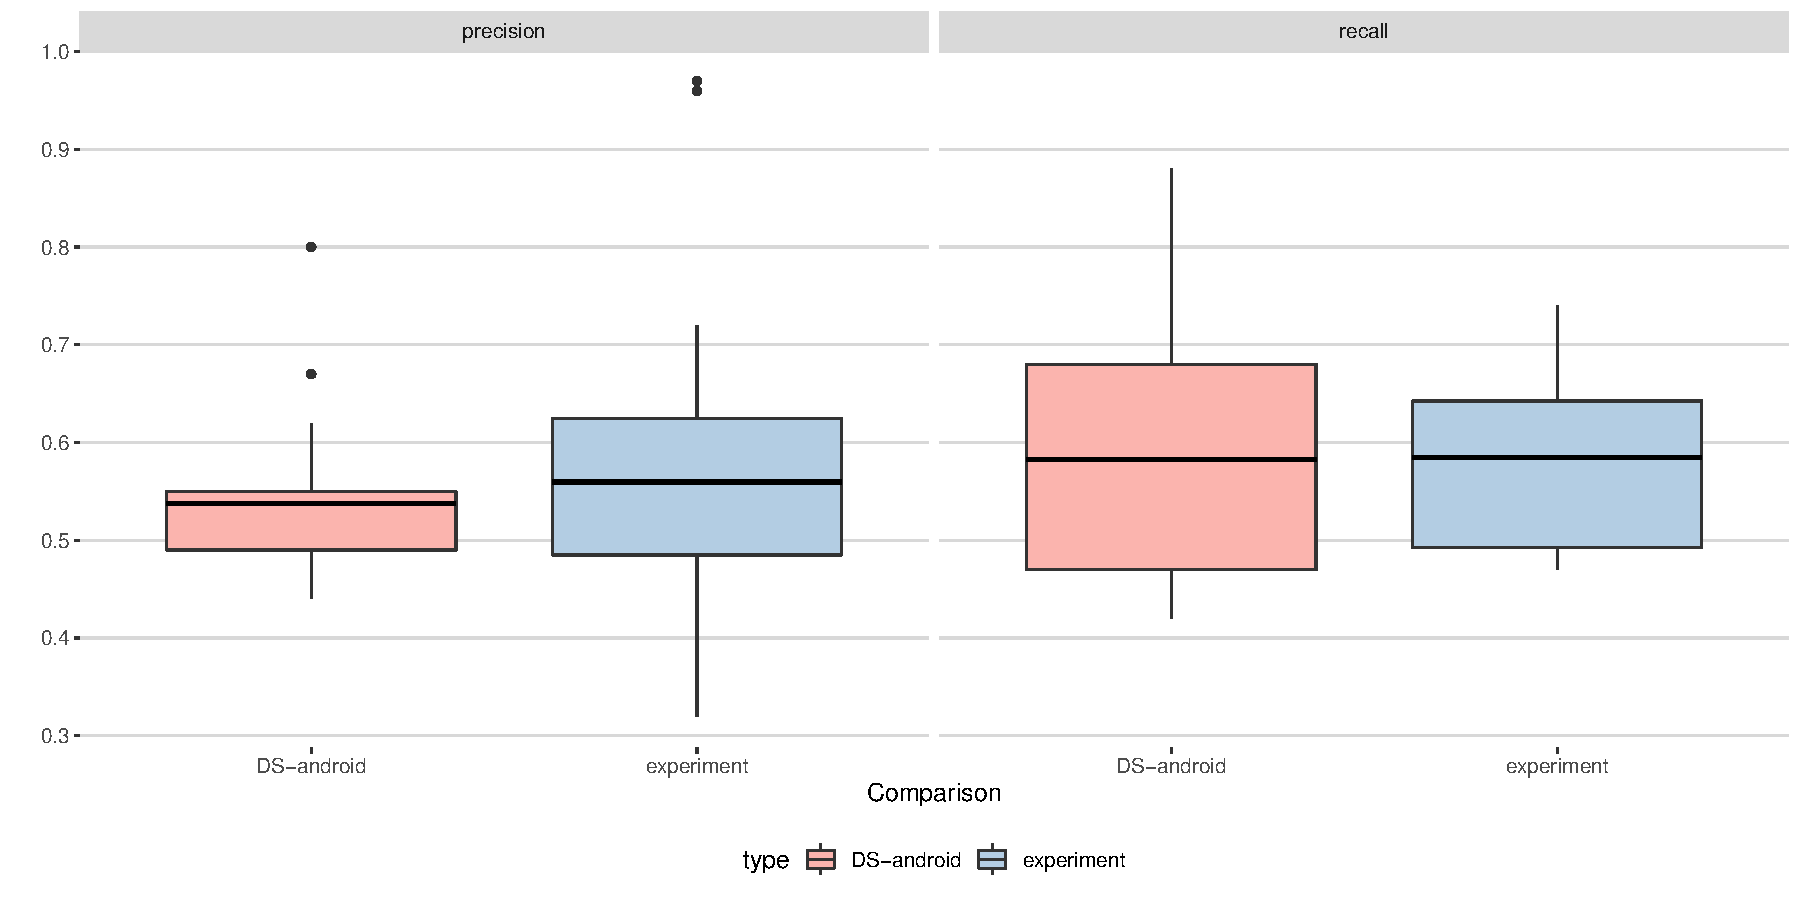
\includegraphics[width=0.95\textwidth]{cp6/eval-comparison.pdf}
    \caption{Boxplots comparing precision and recall values when applying our semantic-based technique to the \acs{DS-python} and the \acs{DS-android} corpora}
    \label{fig:eval-comparison}
\end{figure}
}

